\documentclass[11pt]{article}
\usepackage[margin=1in]{geometry}
\usepackage{amsmath,amssymb}
\usepackage{booktabs}
\usepackage{graphicx}
\usepackage{hyperref}
\usepackage{xcolor}
\usepackage[numbers]{natbib}
\usepackage{caption}
\captionsetup{font=small}
\newcommand{\todo}[1]{\textcolor{red}{[TODO: #1]}}

\title{\textbf{The Diagnostics Release Is the Leak:}\\
Controlled Measurement of Revealed Statistics in Multi-Site GWAS}
\author{Anonymous}
\date{}

\begin{document}
\maketitle

\begin{abstract}
Multi-site genome-wide association studies (GWAS) release not only a final
summary statistic but a stream of intermediate diagnostics---allele frequencies,
$\lambda_{GC}$, the principal-component (PC) spectrum used to correct population
stratification, missingness tables. Privacy-preserving pipelines secure the
\emph{computation} of these quantities while leaving \emph{what is released} to
implementation detail. We measure a question governance proposals assume away:
\emph{how much additional membership leakage does each released diagnostic
carry?} We make one methodological correction---members and non-members are
drawn from the same population, with the attacker's reference panel and the
target non-members kept disjoint from the study (and from each other); the
common shortcut of scoring the attacker's own reference individuals as
non-members inflates measured AUROC by $\approx 0.13$. Under this control the two implemented
non-degenerate canonical diagnostic scores---the study-fitted PC loading matrix
and the allele-frequency summary---are directly comparable: a
projection-distance attack on the study-fitted loading matrix (released with the
PC eigenvalues) reaches $0.88$
AUROC, above the unconditioned allele-frequency summary release ($0.84$ at both
2\,dp and full precision; paired $+0.10$ for the AF$+$PC combination,
95\% CI $[+0.096,+0.110]$ over 25 seeds). PC outperforms unconditioned AF but is
outperformed by conditioned AF (subtracting known calibration members from the
released summary), so we state the AF ordering explicitly rather than claiming a
universal PC dominance. The other canonical
diagnostics we
measure ($\lambda_{GC}$, the leading-eigenvalue ``condition bit'' and the
missingness vector) enter only as limited controls---a per-release-constant
column or an independent random vector---so their near-zero increments limit
those abstract constructions rather than ranking realistic $\lambda_{GC}$,
branch or missingness attacks; we make no ranking against attacks we do not
implement. The observed operating point is not a simulator
artifact: reproducing the small-$(n{\times}M)$ regime the paper locates, real
1000G genomes show the same PC$>$AF ordering within a population (gap $+0.05$ to
$+0.14$ across twelve real cohorts, and on chr1/chr2) and a scale-matched
rerun is consistent with the ordering depending jointly on study size and
composition---at
matched per-group $n$ the PC channel dominates even across populations, and the
AF-first switch appears only as $n$ grows. Among \emph{single} releases, per-site
(per-stratum) allele-frequency release is the largest marginal-frequency channel
($0.96$); two channels outside this canonical set are larger still---an
in-sample-fitted haplotype/LD table ($0.99$) and a membership-correlated
missingness curve (whose $\rho{=}1$ value reaches $1.00$, though a
candidate-only baseline matches it, so it is batch association rather than
release exposure)---and are reported as separate families below. A \emph{raw}
haplotype set is trivially membership-leaking (a member's own haplotypes are
present verbatim), so we treat it as out of the governed set. The PC-spectrum
leak is
attacker-implementable from the release alone (if the study's PC loadings are
shared, as federated PCA shares them); its mechanism is the in-sample-ness of
the study-fitted spectrum (refitting the
loadings on an independent panel collapses the increment to $\approx 0$, an
independent site's basis separates another site's members only at chance, and a
random-basis (eigenvalue-only) projection is at chance while full loadings
recover the leak; fixed, data-independent bases are also at chance, including an
eigenvalue-weighted fixed basis that reuses the released spectrum
(\texttt{s53\_eigbasis.py}, $0.46$--$0.53$ on simulated and real
chr22/chr1/chr2$\times$EUR/EAS/AFR)); a study
eigenvalue ratio of $1.000$ against an independent sample is consistent with the
leak, not evidence against sample-eigenvalue inflation, which both samples would
carry. We
map a site-size $\times$ precision boundary showing leakage collapses with site
size and a coarse rounding cutoff. On real 1000G data the ordering follows the
same boundary: within a single population the study-fitted PC channel dominates
AF (as it does on the simulated panels), and a scale-matched rerun is consistent
with the
AF-first switch depending on total study size as well as composition rather than
on
structure alone. The PC channel
also reproduces under a recombination-realistic msprime demography. A distinct
haplotype/LD channel reaches $0.99$ AUROC and, like the PC channel, is
in-sample-only (it transfers to a fresh panel at chance)---the in-sample-ness of
fitted released objects is a general property, not peculiar to the PC spectrum.
Within a population the PC$>$AF gap is also density-stable, holds under a
stratified permutation null on the same cohorts, and persists to the largest
structure-zero cohort the 1000G panel supports (a study/reference split of a
single super-population at $n_{\text{study}}$ up to $350$).
We further build and stress-test the logic layer of the governance mechanism
itself (a pre-registered reveal manifest, an enforced egress monitor, and a
hash-chained cross-run ledger), quantify the model-dependence of the ordering
(it is approximately decreasing in measured structure under a size-controlled $F_{ST}$ sweep and
crosses at a site-size-dependent measured structure
$\approx0.03$--$0.15$),
turn the sanitized-diagnostics paradox into a controlled result with a
falsification control, and show a released raw haplotype set leaks membership
trivially while a leave-self-out longest-shared-run relatedness statistic does not
separate real unrelated members.
The implication for pre-registered reveal manifests is direct: the diagnostics
that pipelines treat as harmless are exactly the objects that must be
governed---and within our tested projection attack, withholding the study-fitted
loading matrix removes the leak while a random-basis (eigenvalue-only) release
carries none.
\end{abstract}

\section{Introduction}

GWAS power comes from sample size, but genotype data cannot be pooled across
institutions for legal and ethical reasons. The established engineering answer
is to move computation to the data: each site computes summary statistics
locally and only the summaries are combined. This rests on an unstated
premise---that the summaries \emph{are safe to release}. That premise is false
at small site sizes, where allele frequencies and diagnostics can identify
individuals.

Crucially, a real multi-site GWAS does not release a single object. It releases
a \emph{stream}: per-site allele frequencies, $\lambda_{GC}$, the
principal-component (PC) spectrum used to correct population stratification,
missingness and QC tables, and finally association statistics. Secure-computation
work (MPC/HE/TEE federated pipelines) secures how these are \emph{computed}; it
says nothing about which of them are \emph{released}. Governance proposals
therefore argue that releases should be pre-registered and audited. Such
proposals presuppose a fact that has never been measured: \emph{how much
leakage does each released diagnostic carry, and does it add anything beyond the
final statistic?}

This paper measures that. Our contribution is a controlled
leakage-measurement methodology and the finding it produces, not a new
cryptographic primitive.

\paragraph{Contributions.}
\begin{enumerate}
  \item \textbf{The study-fitted PC loading matrix is a strong intermediate
  diagnostic leak.} The released
  study-fitted PC loading matrix supports a projection-distance attack at $0.88$
  AUROC, above the unconditioned allele-frequency summary release ($0.84$ at both
  2\,dp and full precision); combined they reach $0.94$, a paired increment of
  $+0.10$ (95\% CI $[+0.096,+0.110]$ over 25 seeds). A conditioned AF
  attack---valid post-processing of the released summary using known calibration
  members, with no curator refit---is stronger still ($0.94$, above the
  full-study PC), so we state the AF ordering explicitly: the PC release
  out-separates the reference-panel AF attack, though not every AF attacker. The
  remaining canonical diagnostics
  we measure enter only as limited controls (per-release-constant columns or an
  independent random vector), so the comparison is between the PC and AF scores
  at these operating points. Per-site frequency release is the largest
  marginal-frequency channel ($0.96$); an in-sample-fitted haplotype/LD table
  ($0.99$) and a membership-correlated missingness curve ($\le 1.00$, matched by
  a candidate-only baseline, so batch association rather than release exposure)
  are larger still but are
  separate families (Section~\ref{sec:replication}).
  The PC$>$AF ordering also appears on real 1000G genomes in the small-$(n{\times}M)$
  regime the paper locates: within a single population the
  study-fitted PC channel dominates AF (gap $+0.05$ to $+0.14$ across twelve
  small real cohorts, where PC is near-saturated at $k/n{\approx}1/3$, and a
  non-degenerate gap $+0.10$ to $+0.19$ at $n_{\text{study}}$ up to
  $350$ in the fixed-reference pooled arm; Section~\ref{sec:scale}), and a
  scale-matched rerun is consistent with
  the ordering depending on total study size and composition
  (Section~\ref{sec:scale}).
  \item \textbf{Mechanism identification.} The leak is the in-sample-ness of the
  study-fitted spectrum---refitting the loadings on an independent panel
  collapses the increment to $\approx 0$ ($+0.003$), while
  attacker-realistic centering leaves it intact ($+0.10$); sample
  eigenvalues are unchanged (ratio $1.00$). An independent site's fitted basis
  separates another site's members only at chance ($0.50$), and a
  random-basis (eigenvalue-only) projection is at chance ($0.51$) whereas full
  loadings give $0.88$. The attack is
  implementable from the release alone \emph{if the study's PC loadings are
  shared}---as federated PCA shares them so each site can project its own
  genotypes (Section~\ref{sec:mechanism}).
  \item \textbf{A site-size $\times$ precision boundary.} Leakage collapses with
  site size and with a coarse-rounding cutoff; per-site frequency release is by
  far the worst (Sections~\ref{sec:controlled}, \ref{sec:boundary}).
  \item \textbf{Replication and a second channel.} The PC channel reproduces
  under a recombination-realistic msprime demography and on two independent real
  chromosomes (chr1, chr2) at the same sub-AF magnitude with the same
  in-sample mechanism and loadings-granularity ladder; a distinct haplotype/LD
  channel reaches $0.99$ and shares the in-sample-only property
  (Section~\ref{sec:replication}).
  \item \textbf{A built governance layer.} A declarative reveal manifest, an
  egress monitor, and a hash-chained ledger are implemented and stress-tested
  at the release-object level; the ordering's model-dependence is quantified
  (approximately decreasing in measured structure under a size-controlled $F_{ST}$ sweep,
  crossing at a site-size-dependent measured $\approx0.03$--$0.15$), the
  sanitized-diagnostics paradox is upgraded to a controlled result with a
  falsification control, and the tested IBS/LSR channel fails to separate
  unrelated real members (Section~\ref{sec:governance}).
  \item \textbf{A governed-object implication} and the honest scope of the
  governance mechanism (Section~\ref{sec:discussion}).
\end{enumerate}

\section{Related Work}
Secure GWAS computation---MPC, homomorphic encryption, and TEE federated
pipelines---secures the \emph{computation} layer \citep{ostrak2021, aherrahrou2024,
ppgwas2025, fedlmm2025}. secure, collaborative GWAS systems now realize full PCA-based and
LMM-based federated pipelines with cryptographic guarantees
\citep{sfgwas2025}, releasing the study-fitted PC \emph{loadings} so each site
can project its own samples. Our measurement takes that released object as
given and asks what it leaks. Recent work also shows released PCs support full
\emph{data reconstruction}, a strictly stronger attack than membership
\citep{kwatra2023}, and that GWAS summary statistics combined with
high-dimensional phenotype data enable genotype recovery and individual
re-identification under a linear-programming formulation \citep{lan2025}---so
the release object we measure sits inside an active leakage literature we do
not claim to originate. Release-safety work assesses whether a \emph{single}
final release is safe \citep{pascoal2022, igwas2023}; interdependent-release work
checks combined releases of selected SNPs \citep{igwas2023}. The measurement
substrate is the genomic membership-inference literature
\citep{homer2008, sankararaman2009, shringarpure2015, bu2021}, and recent work
warns that reported MI gains can reflect shared cohort traits rather than
membership \citep{popets2026}---the confound our disjoint-negative control
addresses. Outside genomics, a released PCA is already known to leak membership
directly: \citet{zari2022} attack the principal components through a
reconstruction-error score and report stronger leakage for smaller training sets
and more components. Our PC result is not a new attack primitive; we reuse that
released-object leakage in a controlled GWAS setting, and our contribution is the
\emph{comparison} of the intermediate simulated/released objects at matched
operating points (the PC-vs-AF ordering and its site-size/structure boundary),
the requirement that the release name the \emph{loading matrix} as the leaky
object, and the governance layer over the release set. Genomic privacy
\emph{metrics} are known to be non-monotone under
adversary strength and cannot anchor a security claim \citep{wagner2016}, which
is why we report model-specific empirical estimates rather than a budget.
Workflow provenance and transparency logs \citep{prov-o, intoto, rfc6962} record
what happened but cannot pre-authorize an output. Our contribution sits between
these: a controlled measurement of the \emph{intermediate} releases that all of
them leave unmeasured.

\section{Threat Model}
We consider three adversaries. \textbf{A1: honest-but-curious site}---follows
the protocol, tries to infer others' inputs from protocol records; handled by
the MPC layer's simulation security and \emph{not} a claim of this paper.
\textbf{A2: constrained workflow author}---may under-declare or over-precision
releases, use the wrong recipient, or loosen a release condition, but cannot
execute arbitrary code or bypass the mediated runtime. \textbf{A3: adaptive
analyst}---legitimately submits several analyses and uses earlier releases to
build later ones, accumulating leakage; we measure this but make \emph{no}
formal composition claim. We measure A2/A3-visible releases under a
membership-inference adversary holding a disjoint reference panel. We make
\emph{no} data-independent privacy claim; every number is a model-specific
estimate. We separate the syntactic layer (what is released) from the empirical
layer (what it leaks).

\section{Controlled MI Protocol}
\label{sec:controlled}
\paragraph{Data.} We simulate a three-population structured panel
(Balding--Nichols, $F_{ST}=0.08$) and, as an independent,
recombination-realistic cross-check, an msprime three-population demography over
2\,Mb. Each population is split three ways, disjointly: study members, attacker
reference panel, and target non-members. QC keeps variants with minor-allele
frequency in $[0.05,0.95]$ ($\approx 3800$ of $4000$ simulated sites per panel).

\paragraph{Attack.} An allele-frequency likelihood-ratio membership score
($\sum_j \log P(g_{ij}\mid \hat f^{\text{study}}_j) - \log P(g_{ij}\mid
\hat f^{\text{ref}}_j)$). As a structure-only control we project both target
panels onto an independent reference panel's PC basis and score proximity to its
centroid; because both target panels are out-of-sample with respect to that
basis and ancestry-matched to each other, this control isolates the pure
population-structure channel.

\paragraph{Operating point.} Unless stated otherwise, each experiment uses three
ancestries of 300 individuals each per panel (900 study members, 900 attacker
reference, 900 independent non-members from the same three ancestral
populations) and 4000 simulated sites ($\approx 3814$ passing QC;
site-to-member ratio $\approx 4.2$). Real-data numbers use the 1000 Genomes
panels described in Section~\ref{sec:boundary}. Seeds are fixed per experiment
(5 for the frontier and mechanism, 3 for the intermediate-reveal table, 2 for
the boundary and dimension sweeps; the paired-significance study uses 25 seeds,
the real-data orientation and mechanism studies 20 splits, the crossover map
12 seeds per cell, the multi-chromosome replication 20 splits per chromosome,
the site-size sweep 8 seeds per cell, the msprime/haplotype studies 5 seeds, the
fixed-basis probe / second-haplotype / real size-ladder studies 5 splits or seeds
per cell, the
$F_{ST}$ sweep 15 seeds per cell, and the admixture study 10 seeds per setting);
uncertainties are reported as bootstrap CIs where the effect is small.

\paragraph{Methodological note: the self-reference bias.} The common shortcut
scores the attacker's own reference individuals as non-members. Because those
individuals are pulled toward $\hat f^{\text{ref}}$, the test becomes a
symmetric two-panel distinguishability test and overstates the effect. Quantified
directly on the same panels (5 seeds, full-precision AF release), the biased
protocol yields AUROC $0.976$ versus $0.845$ for the disjoint protocol---an
inflation of $0.132$ ($\approx 0.13$ AUROC). We therefore use a third, disjoint
non-member panel and report corrected numbers throughout; this control-design
caution is one of the paper's methodological takeaways.

\begin{table}[t]
\centering
\caption{Release-precision frontier (disjoint non-members, 5 seeds). The
ancestry/structure-only control---both target panels projected onto an
independent reference panel's PC basis---is at chance ($0.502$) at every tier;
per-ancestor AUROC is uniform (F5: 0.860/0.849/0.851). The last column is the
\emph{mean of the per-seed bootstrap bounds for TPR@1\%}, not a confidence
interval for the 5-seed mean.}
\label{tab:frontier}
\begin{tabular}{lccc}
\toprule
Tier (what is released) & AUROC & TPR@1\% & 95\% CI \\
\midrule
F2 top-200 SNPs & 0.590 & 0.023 & [0.009, 0.044] \\
F4 all SNPs, AF 1 dp & 0.622 & 0.031 & [0.014, 0.054] \\
F3 all SNPs, AF 2 dp & 0.840 & 0.183 & [0.119, 0.255] \\
F5 all SNPs, AF full & 0.845 & 0.193 & [0.132, 0.254] \\
F5 per-site AF & 0.964 & 0.588 & [0.490, 0.696] \\
\bottomrule
\end{tabular}
\end{table}

\section{The Diagnostics Release Dominates}
\label{sec:mechanism}
We write the release tiers of Table~\ref{tab:frontier} as \textbf{F}$n$ (final
summary release at increasing precision/visibility) and the intermediate
diagnostics as \textbf{M}$n$ (M0 none; M1 $\lambda_{GC}$; M2 PC spectrum; M3 a
random missingness vector; M4 the leading eigenvalue as a stand-in for a hidden
condition bit). ``Intermediate'' means released \emph{before} the association
statistic, as a workflow diagnostic; the per-site frequency release (F5
per-site) is itself an intermediate object but is reported separately as the
largest marginal-frequency single channel. We add the PC-spectrum diagnostic to the attack as
per-target features (projection distance to the study centroid, and $|$PC1$|$
alignment), evaluated by a cross-validated logistic meta-attack with disjoint
negatives. Among these \emph{implemented} scores the PC channel is the only one
that moves the attack; M1 ($\lambda_{GC}$) and M4 (the leading eigenvalue) are
per-panel constants---identical for every individual in a release---so they
cannot enter a per-individual classifier, and M3 is an independent random
vector, so its feature is a random-projection control. The negligible increments
of M1/M3/M4 therefore show that \emph{these constructed controls} add nothing to
this attacker, not that a realistic $\lambda_{GC}$-, branch-, or
missingness-based attack is weak.

\begin{table}[t]
\centering
\caption{Marginal leakage of intermediate reveals (disjoint negatives, 3
seeds). M1/M4 are per-panel-constant columns and M3 is a random-vector
projection---limited controls, not realistic attacks of those channels. The
PC-spectrum increment is confirmed at 5 seeds (Section~\ref{sec:mechanism}).}
\label{tab:marginal}
\begin{tabular}{lcc}
\toprule
Feature set & AUROC & $\Delta$ vs final-only \\
\midrule
final release only & 0.844 & --- \\
$+\lambda_{GC}$ (const) & 0.844 & $0.000$ \\
$+$ eig1 (const) & 0.844 & $0.000$ \\
$+$ missingness (rand) & 0.844 & $0.000$ \\
$+$ \textbf{PC loadings} & \textbf{0.942} & $\mathbf{+0.098}$ \\
\bottomrule
\end{tabular}
\end{table}

\paragraph{Mechanism.} Projection distance alone gives $0.881$ AUROC---above
both AF summary releases ($0.840$ at 2\,dp, $0.845$ at full precision); $|$PC1$|$
alone is at chance ($0.501$). Refitting the loadings on the attacker's reference
panel (both target panels then out-of-sample) collapses the increment to
$\approx 0$ ($+0.003$). Centering all targets by the public study mean leaves
the increment intact ($+0.09$ to $+0.12$, mean $+0.10$). The top-10 eigenvalues
of the study and an independent sample are equal (ratio $1.000$), which shows the
release does not report inflated study eigenvalues relative to an independent
sample; it does not by itself exclude sample-eigenvalue inflation (both samples
could carry it), so we attribute the leak to the study-fitted \emph{directions},
a claim the transfer test above supports directly. Note the
sign: members sit systematically \emph{farther} from the study centroid than
non-members, because the study-fitted PCs are tuned to the members' variance---
so the study-fitted PC-distance attack scores $\approx 0.12$ with the naive
orientation and $0.88$ with the flipped orientation (the meta-attack learns the
sign, as an adaptive adversary would); we report it as $0.88$, which is the
orientation an adversary would use. A within-ancestry
label-permutation control returns chance ($0.486$).

\paragraph{Paired significance and an auxiliary-information control.} Re-running
the comparison on 25 seeds with the
orientation calibrated on a \emph{held-out} half of the labels (so the reported
test AUROC uses no test-side label information), the calibrated PC channel beats
the AF summary release on every seed ($0.879 \pm 0.009$ vs $0.832 \pm 0.021$;
paired mean gap $+0.046$, 95\% CI $[+0.037,+0.055]$; paired $t$ / Wilcoxon /
sign tests all $p<10^{-4}$), and the logistic combination beats AF by $+0.103$
(95\% CI $[+0.096,+0.110]$). The train-calibrated orientation is the
members-farther direction on 25/25 seeds, agreeing with the mechanism paragraph
above.

The calibrated PC channel and the calibrated logistic combination both use the
known membership of the train half, so we also give the AF channel the same
known-\emph{member} side information: subtract the known calibration members'
genotypes from \emph{the released} study AF and score against the residual
frequency for both classes with disjoint negatives (\texttt{s10\_paired.py},
\texttt{af\_conditioned}). This is valid attacker post-processing of the original
release, not test-label leakage. It reaches $0.941 \pm 0.012$, \emph{above} the
full-study calibrated PC ($0.879 \pm 0.009$) on 25/25 seeds, and above the
logistic AF$+$PC combination ($0.935$). So within this S10 comparison the
conditioned AF attack has the highest mean AUROC among the attacks on the pooled
AF release and the original PCA release (it beats the combination on 19/25
seeds---a higher mean, not an every-seed advantage), and the
headline PC$>$AF ordering is against the \emph{unconditioned} AF baseline
($+0.046$, 95\% CI $[+0.037,+0.055]$). We do not extend the conditioned-AF
result to the real-data experiments, where it was not evaluated.

A natural follow-up refits the PCA on the same remaining panel; that is a
\emph{curator} action (it changes the released object, not an attacker
post-processing) and is a smaller-cohort release comparison, reaching
$0.964 \pm 0.006$ (\texttt{pc\_conditioned}; the orientation is reused from the
training-half calibration, positive on every seed). It is not an attack on the original
release: the residual mean is reconstructable from the released statistics, but
the refitted loading matrix is not, so this comparison does not spend the same
attacker information as the AF residual. The member-only leave-own-out residual
(subtracting the scored member's own genotype before scoring it) is not a
deployable attack---choosing that branch uses the membership being
predicted---and collapses to $0.429$; we report it only as a mechanism reading.

\paragraph{The leak is in-sample-ness, not a transferable structure channel.}
Splitting the study into two disjoint sites A and B and scoring each site's
members against the shared non-members, a site's release-fitted basis separates
its \emph{own} members at $0.88$ but the \emph{other} site's basis separates
them only at chance ($0.50$); a swapped null (scoring site B's members with site
A's basis) is likewise at chance ($0.51$). The channel is the released basis
being fit on the very individuals it is used to test; it does not transfer to a
fresh site. The same test on \emph{real} 1000G chr22 (20 four-way splits of two
disjoint sites plus a shared non-member set) reproduces it: a site's own basis
separates its members at $0.685 \pm 0.015$, but the other site's basis gives
$0.516 \pm 0.013$ and a swapped null $0.516 \pm 0.010$---so the in-sample
mechanism holds on real data as well, at the smaller real-data magnitude.

\paragraph{The leak needs the loadings, not the eigenvalues.} Releasing only the
top-10 eigenvalues (with an attacker-substituted random orthonormal basis)
leaves this projection channel at chance ($0.51$); releasing top-$k$ loadings
recovers it
monotonically ($k{=}1$: $0.53$, $k{=}3$: $0.65$, $k{=}5$: $0.74$), and the full
top-10 loadings give $0.88$. Withholding the loading matrix removes this
projection attack; the random-basis result is a specific (eigenvalue-only
projection) ablation, not a proof that no eigenvalue-dependent attack exists, and
fixed, data-independent bases---including one weighted by the released eigenvalue
spectrum---are also at chance
($0.46$--$0.53$ on simulated and real chr22/chr1/chr2$\times$EUR/EAS/AFR), so
a purely eigenvalue-informed fixed basis does not recover the leak.

\paragraph{The structure control is not a no-op.} The reference-fitted projection
control returns $0.502$ on ancestry-matched members/non-members---its expected
null---but rises to $0.63$ when the same statistic is asked to separate two
genuinely different ancestry groups, confirming it responds to a real structure
signal rather than being inactive.

\paragraph{Dimension dependence and the PC$-$AF crossover.} We map the paired
increment (PC$-$AF, PC orientation train-calibrated) over a
per-population-group $\times$ marker-count grid (Fig.~\ref{fig:pc}(c); the
population group has $400/800/1600$ simulated individuals, from which the study
panel is a $0.3$ fraction per stratum, i.e.\ $360/720/1440$ study individuals
over three strata). The increment
is positive throughout, peaks near the sparse-marker/small-panel corner
($+0.16 \pm 0.04$ at $360$ study individuals, $500$ markers) and shrinks toward denser
marker sets, crossing to $\approx 0$ only at the far corner
($1440$ study individuals, $8000$ markers: $-0.01 \pm 0.01$), where the AF attack is
already near saturation at $0.86$. The PC channel thus overtakes AF
in the small-panel regime and loses to it only when the AF attack is already
near saturation---consistent with the earlier nine-point sweep, now with the
crossover located explicitly.

\begin{figure}[t]
\centering
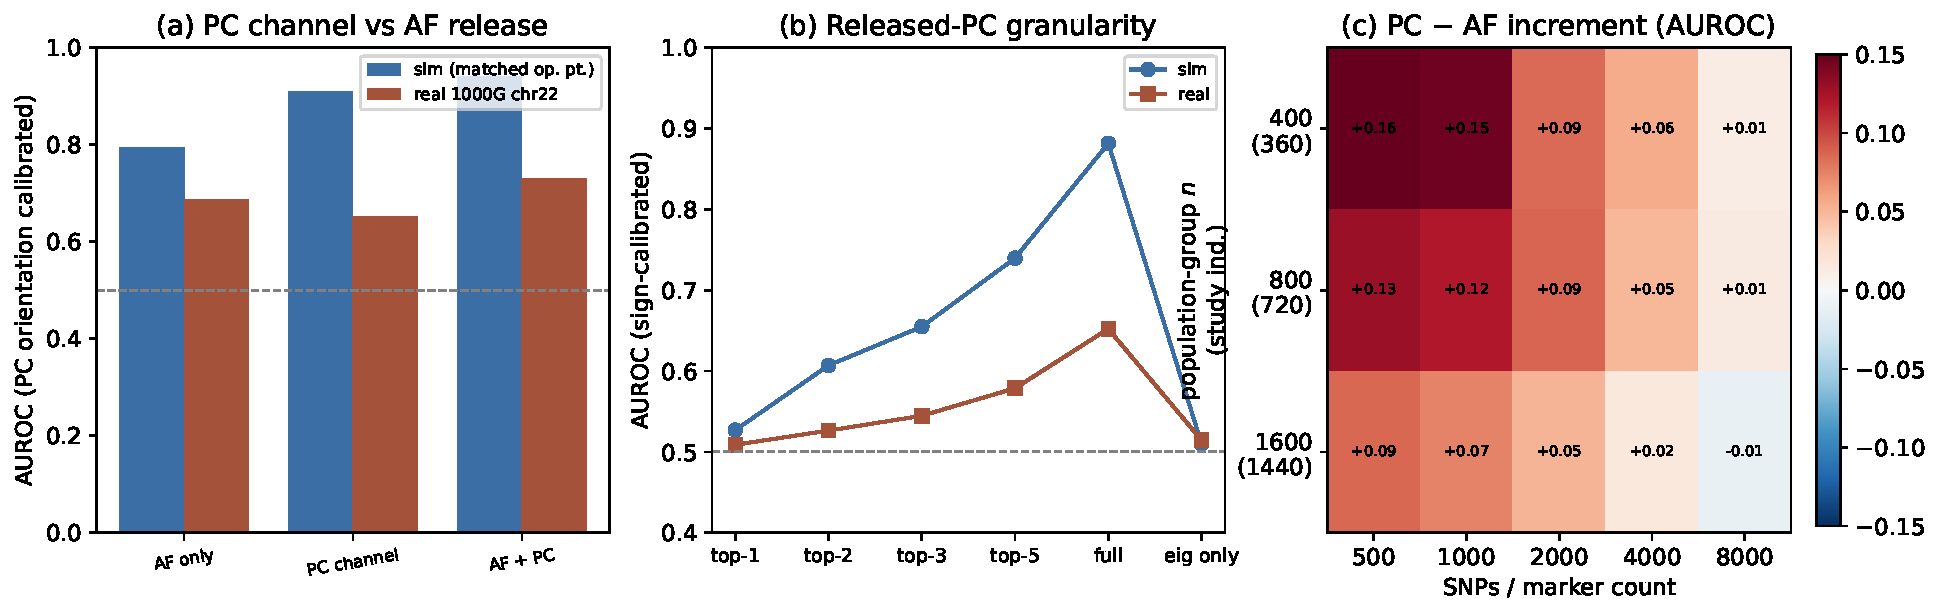
\includegraphics[width=\textwidth]{figures/fig5_pc_channel.pdf}
\caption{The PC channel. (a) Orientation: on the matched simulation the
calibrated PC channel dominates AF; on real 1000G chr22 it is smaller than AF
and its sign-calibrated value sits below the AF release. (b) Released
granularity: the sign-calibrated AUROC rises with the number of released
loadings and is at chance for an eigenvalue-only (random-basis) release, on both simulation and
real data. (c) Paired PC$-$AF increment over the panel-size $\times$ marker
grid; positive in the small-panel regime, crossing to $\approx 0$ only when AF
saturates.}
\label{fig:pc}
\end{figure}

\paragraph{Robustness across functional forms.} The frontier is not specific to
the likelihood-ratio functional: on the same panels, a correlation-form attack
($0.833$) and a cross-validated learned-deviation attack ($0.832$) track the
AF-LRT ($0.845$) at full precision, and at 1\,dp the correlation/deviation forms
retain more signal ($0.660/0.659$) than the LRT ($0.622$)---the LRT is the more
rounding-fragile functional. The PC-diagnostic channel ($0.882$) remains above
all three at every tier.

\section{Site-Size and Precision Boundary}
\label{sec:boundary}
\begin{table}[t]
\centering
\caption{TPR@FPR$\le$1\% by individuals-per-site and AF precision (disjoint
negatives).}
\label{tab:boundary}
\begin{tabular}{lccc}
\toprule
n/site & AF 1 dp & AF 2 dp & AF full \\
\midrule
50 & 0.270 & 0.993 & 0.993 \\
100 & 0.183 & 0.745 & 0.723 \\
200 & 0.062 & 0.307 & 0.301 \\
400 & 0.040 & 0.133 & 0.136 \\
800 & 0.015 & 0.038 & 0.042 \\
\bottomrule
\end{tabular}
\end{table}
Leakage collapses with site size and there is a coarse/fine cutoff: rounding to
1\,dp reduces it sharply while full and 2\,dp precision behave nearly
identically, so the operative lever is the cutoff, not unbounded precision.
An independent msprime demography (weakly structured, 2\,Mb,
recombination-realistic) reproduces the level (AUROC $0.642$ at full precision,
$0.649$ at 1\,dp) but not the rounding benefit: at that operating point the
quantization effect is within noise. We report this honestly---it is consistent
with the saturation reading, in which the benefit comes from crossing the
coarse cutoff rather than from finer rounding at the structured-population
operating point.

\paragraph{Real data.} The same protocol on \emph{real} released allele
frequencies (1000 Genomes Phase-3 chr22, three super-population pseudo-sites
EUR/EAS/AFR, each split three ways disjointly, MAF $[0.05,0.95]$,
distance-thinned at a 15\,kb window; averaged over 5 random three-way splits)
reproduces the ordering with smaller magnitudes: AUROC $0.684$ (full AF), $0.681$
(2\,dp), $0.564$ (1\,dp), $0.640$ (top-200), and $0.808$ for per-super-population
release ($\pm 0.009$--$0.014$ across splits); the reference-basis structure
control is at chance ($0.504$). The qualitative frontier---per-population $>$
full/2\,dp $>$ 1\,dp/top-k---holds on real data. We note honestly that the
smaller real-data magnitudes do \emph{not} have a simple explanation: the real
chr22 panel is, if anything, \emph{more} structured than the simulated panels
(between-super-population $F_{ST}$-like statistic $\approx 0.10$ on the full
chromosome vs $\approx 0.05$ simulated; chr1 and chr2 are higher still,
$\approx 0.14$ and $0.11$; the top-10 PCs capture $0.26$ of total genetic
variance vs $0.14$ simulated; both computed in \texttt{s15\_controls.py} and
\texttt{s20\_extra.py}, the latter on a 2000-marker subset), so ``the real
panel is less structured'' is the wrong
explanation. The plausible cause is that
the real top PCs are dominated by super-population structure that members and
non-members share equally, leaving a smaller \emph{in-sample-ness} share for the
attack to exploit; we flag this as a hypothesis rather than a measured result.

\paragraph{Real-data PC channel.} The released study-fitted PC channel is
\emph{present but sub-dominant} on real data, unlike in the simulation. Running
the S9 orientation study on real 1000G chr22 at a matched operating point
($450$/panel, $1363$ SNPs) over 20 splits: the calibrated PC channel reaches
$0.652 \pm 0.014$ and the AF-only release $0.688 \pm 0.026$---so the PC channel
sits \emph{below} AF on real data, where in the matched simulation the
calibrated PC channel is $0.910$ and AF $0.794$. The direction of the PC channel
is the same on real data as in simulation (members sit \emph{farther} from the
centroid; the calibrated-vs-naive orientation is the same on 20/20 splits), so
the discrepancy is magnitude, not direction. The granularity structure also
replicates: on real data the calibrated channel rises with the number of
released loadings ($k{=}1$: $0.509$, $k{=}3$: $0.545$, $k{=}5$: $0.579$, full
$0.652$) while an eigenvalue-only (random-basis) release is at chance
($0.515$)---the tested projection leak needs
the loading matrix on real data too, it is simply weaker. Added on top of the AF
release, the real-data PC channel gives a small but consistent increment
($+0.043$, 95\% CI $[+0.033,+0.053]$, positive on 20/20 splits, paired
$t$-test $p=1.3\times10^{-7}$; the two channels are partly redundant, so the
increment is smaller than either channel alone). Combined with the real-data
mechanism test above, the picture is consistent: the same in-sample-ness
mechanism, at smaller magnitude at the mixed real operating point (a magnitude
difference governed by study size and structure, Section~\ref{sec:scale}). We
therefore scope the claim: \emph{relative to the unconditioned AF-LRT baseline,
the diagnostics release (the study-fitted PC
loading matrix) is the stronger of the two implemented non-degenerate canonical
diagnostic scores in the small-$(n{\times}M)$ regime---which
includes single-population real cohorts, where the PC diagnostic dominates the
AF release---while once study size and structure grow the AF release leads}, and
we report the operating-point dependence rather than tuning it away.
(The real-data top-200 tier is selected by
$|$AF$-$refAF$|$ rather than by association $p$-value, because the real release
has no phenotype; this is a proxy for a released interesting set.)

\section{Replication and a Second Channel}
\label{sec:replication}
We stress the two scoping caveats---real data is chr22-only, and the PC channel
was only measured on the parametric simulator---by replicating on two
independent chromosomes and on a recombination-realistic simulator, and by
adding a genuinely distinct attack family.

\paragraph{Two independent real chromosomes.} Running the orientation,
mechanism, and granularity studies on chr1 ($5257$ markers) and chr2 ($4664$
markers), each with 20 disjoint three-way splits (Fig.~\ref{fig:rep}(a)):
chr1 gives AF $0.768 \pm 0.045$, calibrated PC $0.675 \pm 0.016$, AF+PC
$0.805$; chr2 gives AF $0.752 \pm 0.046$, PC $0.689 \pm 0.015$, AF+PC $0.799$.
The chr22 ordering replicates: on \emph{both} new chromosomes the PC channel is
\emph{below} the AF release but adds a consistent increment. The mechanism also
replicates---a site's own basis separates its members (chr1 $0.73$, chr2
$0.74$) while the other site's basis is at chance ($0.51$) and a swapped null
is at chance ($0.51$)---and so does the granularity ladder (full $0.675/0.690$,
monotone in $k$, eigenvalue-only $0.516/0.514$). That the same
in-sample-ness mechanism and loadings-granularity ordering hold on three
independent chromosomes strengthens the real-data reading beyond the single
chr22 result.

\paragraph{Recombination-realistic simulator.} On an msprime
three-population demography (real recombination, $5$\,Mb, realistic site-
frequency spectrum), the PC channel is again above AF (calibrated PC
$0.691 \pm 0.013$ vs AF $0.627 \pm 0.015$; Fig.~\ref{fig:rep}(b)), with the same
granularity ladder (top-1 $0.524$, top-5 $0.621$, full $0.691$, eigenvalue-only
$0.512$). The held-out-site mechanism replicates under an ancestry-matched
within-population split (in-sample $0.729 \pm 0.015$, out-of-sample
$0.510 \pm 0.010$, swapped null $0.518 \pm 0.012$). The PC-dominance and the
mechanism are therefore not artifacts of the parametric simulator's injected LD
blocks.

\paragraph{A haplotype/LD channel.} Our AF-LRT, correlation, and learned-
deviation attacks all consume per-SNP marginals. A distinct family uses the
\emph{joint} distribution of adjacent markers (the within-window haplotype
structure): score a target by $\sum_j [\log P_{\text{study}}(g_j,g_{j+1}) -
\log P_{\text{ref}}(g_j,g_{j+1})]$ over adjacent pairs, at the same operating
point (900/900/900, $4000$ markers, 5 seeds). This reaches $0.990$ AUROC---above
every marginal channel---and, crucially, it is \emph{in-sample-only}: fit on
disjoint panels that saw neither the study nor the targets, it transfers at
chance ($0.487$; Fig.~\ref{fig:rep}(c)). The \emph{released joint LD table} is a
hypothetical release object (a workflow could publish pairwise $r^2$/haplotype
frequencies as a QC diagnostic), so we report it as a family bound rather than a
standard release. The in-sample-ness of a fitted released object is thus a
general property of the release, not peculiar to the PC spectrum. A leave-self-out
longest-shared-run relatedness diagnostic is reported in
Section~\ref{sec:scale}, where it is at chance on
three chromosomes at physical length.

\paragraph{The site-size regime.} At realistic site sizes with $10{,}000$
markers and 8 seeds (Fig.~\ref{fig:rep}(d)), the PC channel's dominance over AF
does not survive: at $n=1200$ it is roughly tied (AF $0.909$, PC $0.896$) and at
$n=3000$ AF leads (AF $0.807$, PC $0.745$). The $+$PC increment is essentially
unchanged ($+0.055$--$+0.056$), so the \emph{combination} stays above AF
($0.966/0.862$) and the PC channel still contributes---but the ordering
statement is genuinely an operating-point property. This is consistent with the
crossover map: PC-dominance is a small-site phenomenon, and at the site sizes
real biobanks report the AF release already saturates.

\begin{figure}[t]
\centering
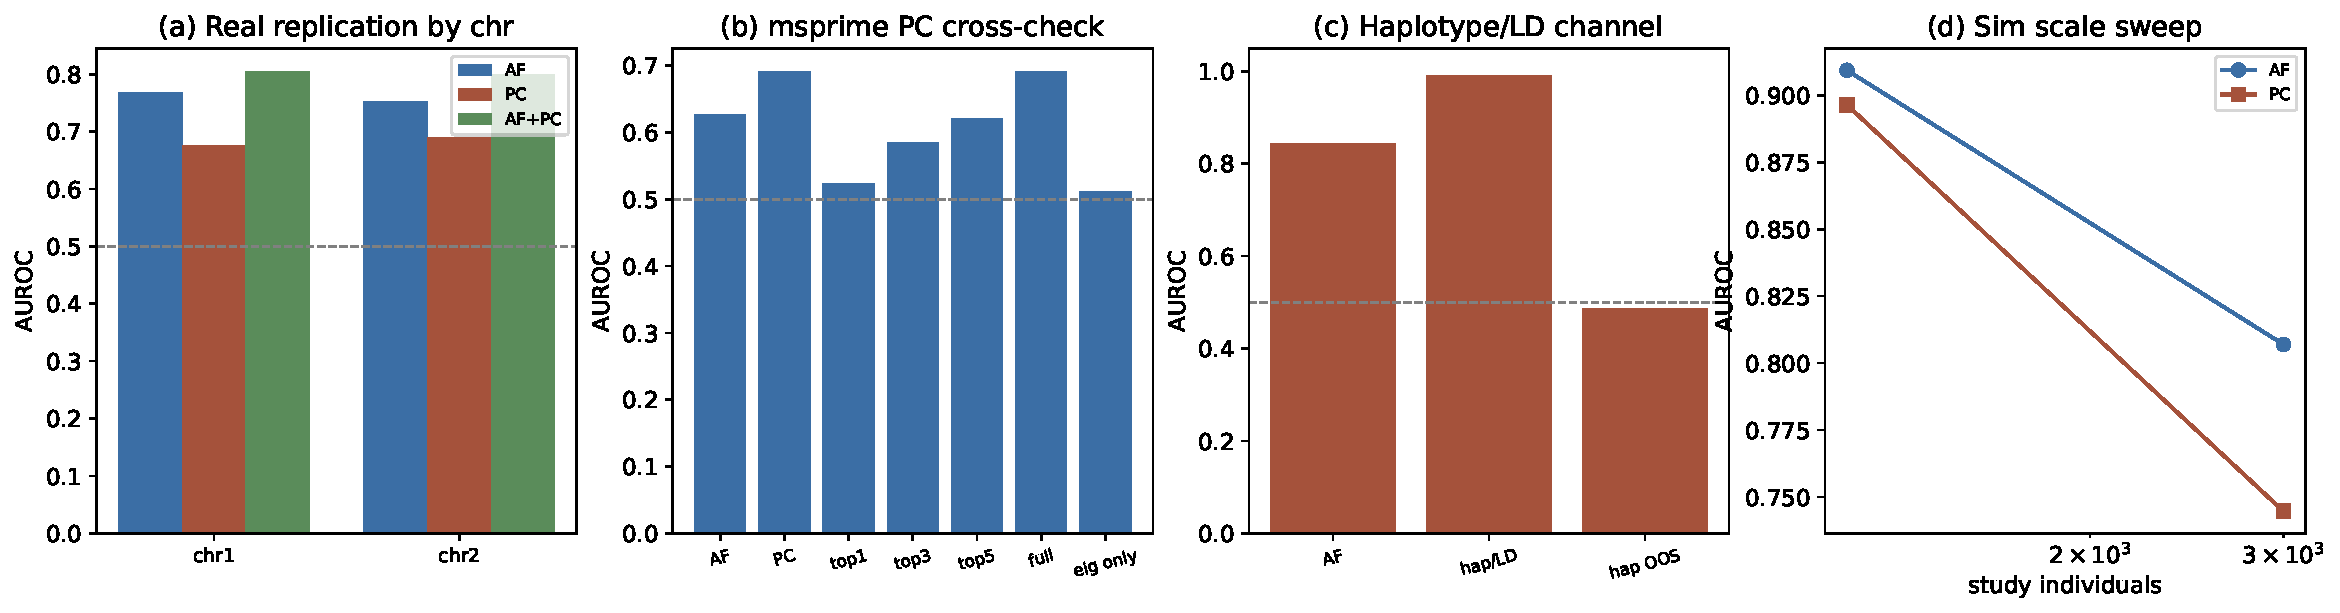
\includegraphics[width=\textwidth]{figures/fig6_replication.pdf}
\caption{Replication and a second channel. (a) Real replication on chr1 and
chr2: the PC channel is below AF but adds a consistent increment, replicating
the chr22 ordering. (b) msprime cross-check: PC above AF with the same
granularity ladder. (c) A haplotype/LD channel reaches $0.99$ but transfers to
a fresh panel at chance---in-sample-only, like the PC channel. (d) Site-size
sweep ($M{=}10{,}000$): the $+$PC increment is stable ($+0.06$) but PC no longer
dominates AF at $n\ge 1200$.}
\label{fig:rep}
\end{figure}

\section{Building and Stress-Testing the Governance Layer}
\label{sec:governance}
The paper argues for pre-registered reveal manifests, enforced egress, and
cross-run auditing; here we build \emph{both} the release-object layer and the
sole-egress binding of that mechanism and stress-test them. The prototype
(\texttt{code/governance.py})
provides (i) a declarative, content-hashed, versioned \emph{manifest} of the
quantities a run may release, each with a semantic type, precision, recipient,
and condition; (ii) an \emph{egress monitor} that wraps the study's release
objects and can emit only declared quantities, coerced to the declared precision
(decimal rounding, top-$k$ truncation, binning, threshold-bool); and (iii) a
tamper-evident \emph{hash-chained ledger} storing a value hash per release
(never raw values) plus the cross-run relations refinement / condition-loosening
/ duplicate / recipient-expansion.

\paragraph{A built sole-egress binding.} The monitor above is a plaintext
library call: a study author who simply does not call \texttt{release} writes a
withheld quantity straight out. We first demonstrate the bypass as a positive
control (\texttt{code/s39\_enforcement.py}): the same exfiltration line
(\texttt{open(...,'wb').write(loadings)}) succeeds against the library prototype
and the withheld loadings land on disk (3/3 seeds). We then close it with a
minimal process-isolation runtime (\texttt{code/enforce.py}): the study
computation runs as a child process whose singleton sanctioned egress route is
one pre-opened pipe descriptor wired to the parent's \texttt{EgressMonitor}; its
stdout and stderr are discarded (\texttt{/dev/null}), and a
startup PEP-578 audit hook denies write-opens, socket creation and
datagram/stream sends, subprocesses, and
\texttt{ctypes} loading. Under the isolated runtime the same natural-egress
write is blocked (3/3 seeds, the leak file is never created), a sanctioned push
of an undeclared object is blocked by the parent monitor (the second enforcement
point), a declared release still flows and its hash chain verifies, and the
transported governed release lands at the \S\ref{sec:governance} governed tier
(AF $0.624$, PC $0.509$). A bounded regression check closes the ordinary-Python
datagram route: the same runtime that blocks \texttt{socket.connect} also denies
\texttt{socket.\_\_new\_\_}\,/\,\texttt{sendto}, and a child that tries an
ordinary UDP \texttt{sendto} to a fixed \texttt{127.0.0.1:9} destination is
stopped at socket creation
(``UDP sendto returned (not blocked)'' never observed, 3/3 seeds,
\texttt{s39\_enforcement.py}). The monitor's release-object API handles the
per-group (dict-valued) AF object directly: permitted full-precision and rounded
(2\,dp) per-group AF releases both flow through \texttt{EgressMonitor.release}
with the ledger chained (3/3 seeds), so the strongest single bundle channel is
supported at the release-object API level. The \emph{isolated} transport is
tested on a fixed declared set (AF, eigenvalues, $\lambda_{GC}$) and on blocking
an undeclared object; it does not yet emit per-group AF through the monitored
release path (per-group AF is serialized and restored in the parent, but is
omitted from the isolated runtime's monitored release loop).
The threat model is the careless study-code author
(ordinary Python, not root, no native code), matching the paper throughout; a
local user with process control and the parent runtime stay in the trusted
computing base. The stated ``no native code'' boundary is itself tested: an
injected \texttt{ctypes.CDLL(None)} call from the child is denied on
\texttt{ctypes.dlopen}\,/\,\texttt{ctypes.dlsym} (3/3 seeds), so the native
loading route does not escape the hook. This turns the one previously argued
mechanism into a built and tested one.

\paragraph{Enforcement.} Under a governed manifest (AF at 1\,dp, eigenvalues
released, loadings/af-by-group/missingness/p-values withheld) the monitor's
outcome matrix on the standard attack injections is: undeclared loadings,
undeclared missingness, undeclared condition bit, recipient expansion, and
condition loosening, all \emph{blocked}; an attempt to emit full-precision AF
into a 1\,dp slot is \emph{coarsened}; the hash chain verifies
(\texttt{s23\_governed.py}). The consequence is the predicted one: the leakage
attacks on the governed release drop from AF $0.845$ / PC-dist $0.882$ to AF
$0.622$ / PC-dist $0.510$ (Fig.~\ref{fig:gov}(b))---i.e.\ the monitor's output
equals the governed tier.

\paragraph{Absolute per-individual exposure.} Every number above is a rank
statistic (AUROC); a privacy reviewer asks what it means for one person. We
re-express the operating points in absolute per-individual terms
(\texttt{s38\_privacy\_metric.py}, 5 seeds): the membership advantage
$A^\ast=\max_t|\text{TPR}-\text{FPR}|$ (the two-sided KS distance between the
member and non-member score distributions), the per-individual
posterior $\rho_i$ from a score-density likelihood ratio, and a resolution-floored
empirical $f$-DP trade-off summary
$\varepsilon_{\text{lb}}(\delta)=\max_\alpha\max\{\log((\text{TPR}(\alpha)-\delta)/\alpha),\ \log((1-\delta-\alpha)/(1-\text{TPR}(\alpha)))\}$
over the two non-trivial branches of the trade-off function $g_{\varepsilon,\delta}$.
It is an in-sample, resolution-floored summary of the observed trade-off,
evaluated over rates at or above their sample
resolutions ($1/n_{\text{neg}}{=}1/n_{\text{pos}}{=}1/900$) and computed
on the same individuals the score was fit on, so
it is a descriptive, resolution-limited summary of the observed trade-off rather
than a release-level guarantee; a false-negative rate floor
($1/n_{\text{pos}}$ in the default reading, or $3/n_{\text{pos}}$---the
rule-of-three upper bound on a zero count---in a conservative reading) keeps the
strict trade-off finite where a single zero observed false-negative count would
otherwise make it infeasible, so the reported values are floored under a stated
convention (the \texttt{valid} flag checks consistency with that convention, not
statistical validity); we do not model
aggregate $k$-anonymity, which is not
well-defined for these releases. The selected comparisons retain their ordering:
the released
loadings give $A^\ast{=}0.61$ and $\varepsilon_{\text{lb}}{\approx}5.0$ at
$\delta{=}0.01$ (the quoted $\varepsilon$ values use the default $1/n_{\text{pos}}$
floor), versus $0.55$/$4.1$ for full-precision AF and $0.19$/$1.1$ at
1\,dp; the reference-fitted-basis and eigenvalue-only controls sit at
$A^\ast{\approx}0.04$, $\varepsilon_{\text{lb}}{=}0.19$--$0.24$ (the $\varepsilon$
summary is not monotone in AUROC across all channels---full-precision AF has the
higher AUROC over AF@2dp but the lower $\varepsilon$---which is why we read it
per-channel rather than as a global ordering). $A^\ast$ is the KS
distance, a distinct quantity from AUROC rather than a rescaling of it. The
metric is not a simulator artefact: re-expressed on
\emph{real} 1000G chr22 and on the semi-synthetic cohort (8 splits; 3 cohort
seeds, \texttt{s44\_individual\_real.py}), the ordering is preserved (real chr22
PC loadings $A^\ast{=}0.27$ below full-precision AF $0.35$ and sitewise AF
$0.58$, matching the real
AUROC ordering; on the cohort AF $0.13$ leads PC $0.04$) and both controls sit at
$A^\ast{\le}0.07$. The $\varepsilon$ summary is descriptive and floored under a
stated convention (default $1/n_{\text{pos}}$; conservative rule-of-three
$3/n_{\text{pos}}$) on every channel, so we read it per-channel rather than as a
statistical bound.

\paragraph{Composition.} Individually manifest-permitted releases compose: a run
sequence ($\lambda_{GC}$, eigenvalues, AF@1dp, AF@2dp, AF full, then the
loadings) has cumulative AUROC $0.941$ vs $0.882$ for the largest single release,
and the union exceeds the max constituent in 5/5 seeds (Fig.~\ref{fig:gov}(c);
the constant $\lambda_{GC}$-only first run sits at the chance baseline $0.50$, as
does its single-release point).
The ledger records a refinement relation at the AF$\to$loadings step; this is
\emph{producer-asserted} metadata (the prototype records and audits relations,
it does not content-infer them), so an anti-composition policy turns the declared
refinement into a pre-registered violation rather than the monitor silently
inferring it.

\paragraph{A multi-object bundle leaks more than its parts.} The composition
result above is a \emph{declared sequence}; a realistic run releases a bundle at
once. Measuring the full aggregate of a constructed bundle
(pooled AF@2dp, per-site AF@2dp, top-10 eigenvalues, $\lambda_{GC}$@2dp, the
per-SNP call-rate table, top-50 $p$-values) with a joint out-of-fold logistic
attacker (\texttt{s40\_bundle.py}, 5 seeds; the classifier is trained on four of
five stratified folds with known membership and scored on the held-out fold, a
separate split from the half-study compositional split that defines the call-rate
table's contributor set: the call-rate table the study
releases is the object the attacker consumes, coarsened at the manifest's
declared 2\,dp), the bundle reaches $0.958$ versus
$0.947$ for the strongest single object (per-site AF), an excess of $+0.011$ in
5/5 seeds. Leave-one-out attribution shows per-site AF is the largest single
contributor (dropping it costs $0.084$), and the excess comes from the
\emph{orthogonal} per-individual channels it combines (per-site AF plus the
call-rate table), not from feature count: stacking a random per-individual
column onto pooled AF leaves the AUROC unchanged ($0.839$); the
per-panel-constant objects (eigenvalues, $\lambda_{GC}$, $p$-values) carry no
per-individual variation and contribute no feature to the evaluated
per-individual attacker (they could still carry candidate-dependent signal in an
attacker we do not implement, so the negative is scoped to the tested attacker).
The bundle is a constructed composition example: its objects do not all share
one contributor set. The genotype-derived objects (pooled AF, per-site AF,
eigenvalues, $p$-values) are fit on the full study; the call-rate table is
averaged over a train half of the study plus all reference individuals (the
contributor split is exposed through the M3 contributor/non-contributor reading
below). The measured excess is therefore an attribution of which object adds
signal, not a claim that a single workflow emits exactly this contributor
composition.
The released call-rate table adds a small conditional increment beyond the
candidate's own call-count information: AF channels plus the candidate-only call
count reach $0.952$, and adding the released-table M3 score raises it to $0.959$
($+0.008$, positive 5/5 seeds; the second manifest gives $0.965{\to}0.971$,
$+0.006$, 5/5), so the released table carries a small gain over the AF channels
plus the candidate's total call count (a specific comparator, not all
candidate-side information).
The M3 call-rate feature scores every member (the released study table is
observable to all of them); restricted to the members who did \emph{not}
contribute to the table its AUROC is $0.511$, so the M3 channel's $0.705$ is
largely the members who are themselves averaged into the released table---we
report both readings.
The excess is not specific to that manifest or to the coarsened comparator:
under a second manifest (per-site AF at \emph{full} precision, eigenvalues,
$\lambda_{GC}$@2dp, call-rate table; pooled AF and $p$-values omitted,
\texttt{s46\_bundle\_manifest2.py}) the bundle reaches $0.970$ against an
\emph{uncoarsened} strongest single object at $0.964$, an excess of $+0.006$
(positive 5/5 seeds; $+0.023$ against the coarsened single object of the first
manifest). So the per-channel analysis under-estimates the bundle, and an
anti-composition clause must cover orthogonal channels, not only the
AF-versus-loadings refinement.

\paragraph{Model-dependence of the ordering.} The PC-vs-AF ordering is not
free-floating: sweeping the simulated $F_{ST}$ from $0.02$ to $0.24$ (three site
sizes, 15 seeds), the PC$-$AF gap decreases at every site
size and crosses zero at a \emph{measured} structure statistic that depends on
site size (the size-resolved crossing brackets are $[0.027,0.052]$ at
$n{=}1600$, $[0.052,0.077]$ at $n{=}800$, $[0.103,0.151]$ at $n{=}300$); a
within-population real cohort ($\text{Fst}\approx0$) sits \emph{before} the
crossing, and the real mixed three-population cohort (measured
$\text{Fst}\approx0.09$ at $n_{\text{study}}{=}450$) sits near parity, i.e.\
\emph{at} the crossing for its size rather than clearly beyond it
(Section~\ref{sec:scale}). The
read is best done in \emph{measured} terms: at nominal $F_{ST}{=}0.08$ the
realized between-group statistic is ${\approx}0.05$, i.e.\ measured $\approx$
$0.63\times$ nominal. The real-data ordering is therefore the same
structure-and-size dependence as the simulated one, evaluated at the real
cohorts' operating points rather than an unexplained discrepancy; the in-sample
mechanism (own-basis $\gg$ other-basis) holds at every point, and it reproduces
on real within-population data at the PC-dominant magnitude
(Section~\ref{sec:scale}). The
decrease is strict at $n{=}800$ and $1600$ (at $n{=}300$ both attacks sit near
ceiling and the gap is within the sweep's tolerance of flat). A Dirichlet
admixture sweep (varying the concentration parameter, which interpolates between
nearly-pure individuals and near-uniform mixes; it does \emph{not} isolate
discrete-vs-continuous structure) again moves the gap with the realized
structure, from $-0.12$ at the most concentrated setting to $+0.10$ at the most
uniform (\texttt{s22\_admixture.py}), i.e.\ the ordering tracks structure
strength rather than the discrete/admixed label.

\paragraph{The sanitized-diagnostics paradox, as a result.} Replacing the
earlier probe-count statistic with one measured on the \emph{released object}
(the attack AUROC of the finest AF the analyst actually sees), and running
seven analyst families over 12 seeds with a quality-parity margin, the paradox
holds in the predicted regime and only there: pre-providing a coarse sanitized
block reduces exposure by $\Delta_E=+0.24$ (95\% CI $[0.23,0.26]$) when the
sanitized precision is coarser than the analyst's stopping precision, and
$\Delta_E=0$ when it is not---while a \emph{null} analyst that needs no
diagnostic shows \emph{no} paradox (the falsification control). The effect is
tightly the exposure-curve difference $\Delta_E=e(p_{\text{stop}})-e(p_{\text{san}})$:
the families set only the stopping rung, and quality is nearly flat in the
chosen $k$ (so parity is a consequence, not a coincidence); moreover the null
family at $p_{\text{san}}\ge2$ shows a \emph{negative} $\Delta_E\approx-0.24$
because a coarser-than-needed sanitized block \emph{is} the leak---the sharp
version of the "precision-gap effect" the prediction names
(\texttt{s25\_paradox.py}).

\paragraph{An IBS window-sharing channel.} The haplotype/LD channel above (0.99) is an
in-sample-fitted joint table---it transfers at chance. A genuinely distinct
identity-by-state (IBS) \emph{window-sharing} attack (the fraction of 8-marker
windows a target matches to any study vs any reference individual; run here on
unphased dosages---the 1000G VCFs are phased, and \texttt{real\_phased.py} loads
the haplotypes, but this arm has not yet exploited H0/H1 separately) detects a
\emph{planted} IBD segment at
$0.866$ but is at chance on unplanted simulation ($0.486$) and on real chr22
($0.463$, below the real AF channel $0.653$; Fig.~\ref{fig:gov}(d)). So the
0.99 adjacent-pair number is a fitted-table artifact, and real haplotype sharing
among unrelated 1000G samples leaks little under the tested statistics---a
characterization of the tested IBS statistic and the leave-self-out LSR
diagnostic, not a bound on the haplotype channel as a whole.

\begin{figure}[t]
\centering
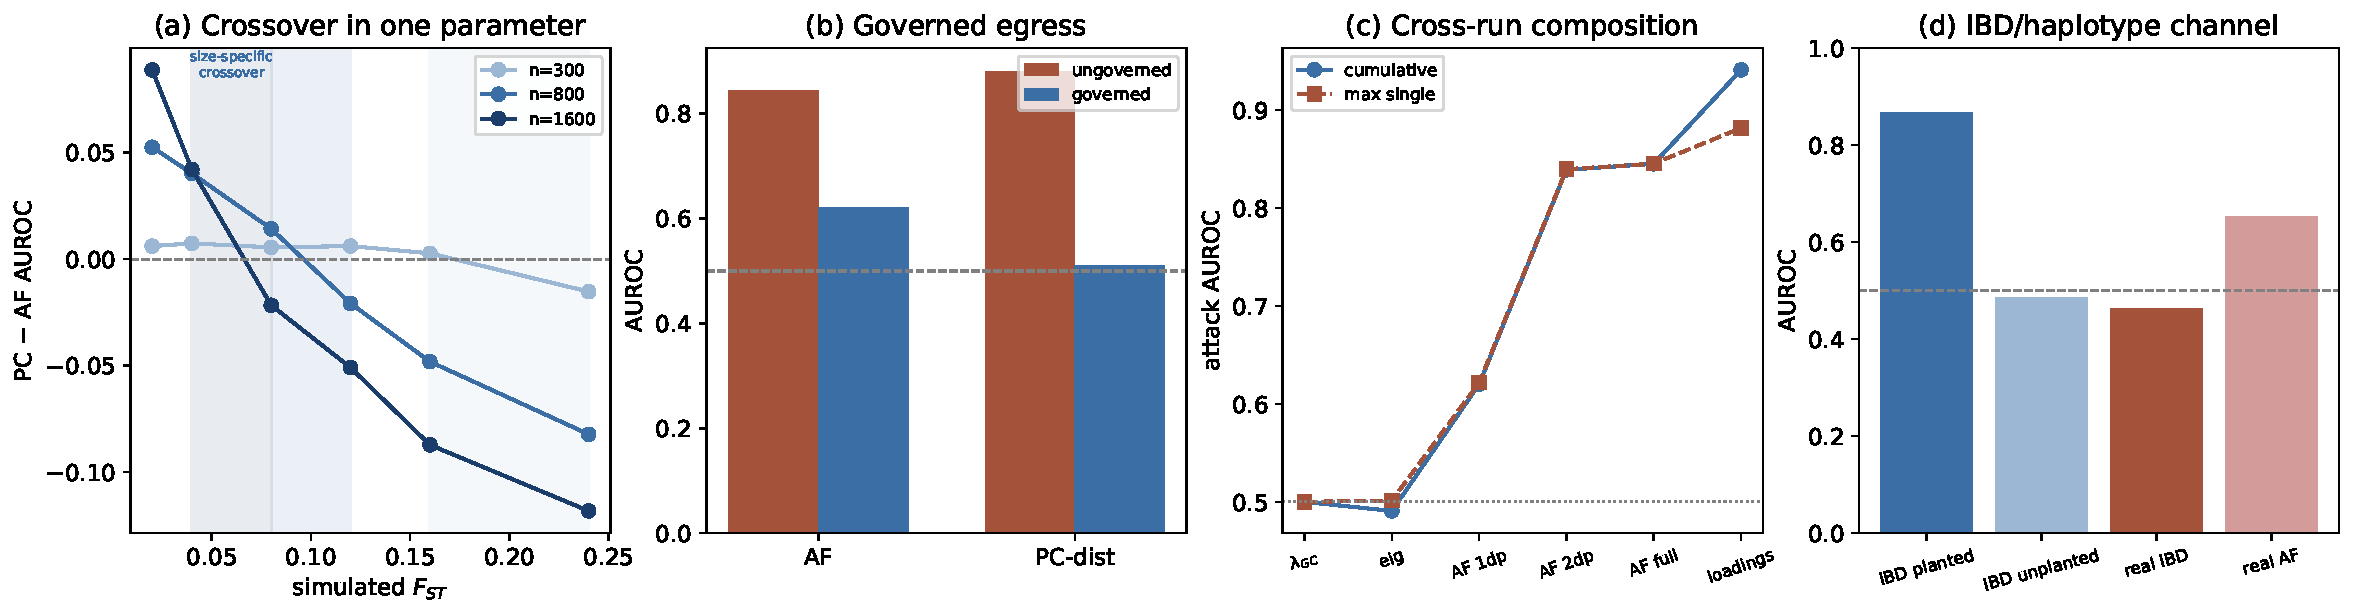
\includegraphics[width=\textwidth]{figures/fig7_governance.pdf}
\caption{Governance layer and model-dependence. (a) The PC$-$AF gap decreases
in simulated $F_{ST}$ (three site sizes) and crosses zero at a
measured structure that depends on site size (measured crossover
$\approx0.03$--$0.15$ across the three sizes; the bands mark the per-size
nominal crossing interval). (b) Governed egress: the monitor's
manifest-permitted release (AF@1dp, loadings withheld) drops the leakage attacks
to the governed tier. (c) Cross-run composition: individually coarsened releases
compose above the largest single release. (d) An IBS window-sharing channel
detects planted IBD but is at chance unplanted and on real data.}
\label{fig:gov}
\end{figure}

\section{Scale, Density, and Ancestry: Where the Ordering Lives}
\label{sec:scale}
The ordering claims above are operating-point properties; a GPU-ported harness
(host-resident int8 panels, blocked exact-Gram PCA on GPU; the governance layer
itself is CPU/plaintext) lets us locate the boundary at
biobank dimensions and retire three data caveats at once.

\paragraph{The boundary is small $(n{\times}M)$.} Sweeping study size and marker
count (Fig.~\ref{fig:scale}(a,b)): at $n_{\text{sp}}{=}500$ (1500 study genomes)
the PC channel leads only below $\sim\!10^4$ markers ($+0.008$ at $M{=}5$k) and
falls behind above it ($-0.02$ at $M{=}10^4$, $-0.03$ at $M{=}5\cdot10^4$); by
$n_{\text{sp}}{=}2000$ AF leads at every $M$ ($-0.03$ to $-0.18$, widening with
$M$); at $n_{\text{sp}}{=}8000$ AF leads
decisively ($0.75$--$0.84$ vs $0.59$--$0.65$). The dominance is thus a
small-study phenomenon, and the AF release saturates first. The mechanism is
unaffected by scale: projecting onto the \emph{reference}-fitted basis collapses
the PC channel to chance ($0.485$--$0.504$) in \emph{every} cell, and the
in-sample gap shrinks monotonically with study size within each Fst column (at
$\text{Fst}{=}0.04$: $+0.51\!\to\!+0.15$; $\text{Fst}{=}0.08$:
$+0.50\!\to\!+0.11$, all at matched $M$).
A denser, small-$n$ sweep (Fig.~\ref{fig:scale}(b)) locates the crossing
directly.

\paragraph{The gaps are real, and tightly so.} A stratified label-permutation
null ($2\cdot10^4$ permutations/cell, permuting within ancestry) puts both
channels far above chance in every cell ($p<5\cdot10^{-5}$), so neither
discrimination is a structure artifact; a paired sweep (three $200$-seed shards
$+$ one $200$-seed run for the slow cells, $600$ seeds on each fast cell) gives
the small-$n$
PC-AF gap as $+0.094$ [$+0.092,+0.096$], $P(\Delta>0){=}1.0$
($600$ seeds), decaying to $+0.009$ [$+0.008,+0.009$], $P(\Delta>0){=}0.94$ at
$M{=}8000$ and turning \emph{negative} ($-0.014$, $P(\Delta>0){=}0.21$,
$200$ seeds) at $n{=}1600$. The exact
$k$-ladder (Fig.~\ref{fig:scale}(c))
is monotone with strictly decaying increments ($+.13,+.07,+.06,+.04,+.04,+.03,
+.02,+.02,+.01$ for $k{=}1\ldots10$ on the simulator)---still climbing
slightly at $k{=}10$, so we report it as saturating only in the sense that the
per-$k$ increment has fallen to $\lesssim0.02$; an eigenvalue-only control
stays near chance on the simulator, on real chr22/chr1/chr2
(s48/s50 $0.38$--$0.60$; s49 $0.42$--$0.50$), on
msprime
($0.50$--$0.53$), and in every cell of the biobank-scale grid
($0.497$--$0.511$)---the leak is in the loadings at every tested corpus and
scale.

\paragraph{Density does not reverse it.} Raising real marker density by $20\times$
(chr22: $2.2$k$\to$48k; chr1/2: $13$k$\to$264k markers;
Fig.~\ref{fig:scale}(d)) leaves the PC channel flat ($0.66$--$0.67$) while AF
\emph{rises}, so the PC-AF gap widens rather than closes.

\paragraph{Where the ordering lives on real genomes.} Running the identical
attack code on real 1000G cohorts of varying composition
(\texttt{s48\_real\_structure.py}, chr22, 5 split seeds per cohort), the
study-fitted PC channel \emph{dominates} AF within a single population and
\emph{reaches parity or falls below} it once population composition broadens
\emph{and} study size
grows: twelve single-population cohorts all give $\text{PC}>\text{AF}$ (gap
$+0.051$ to $+0.136$; GBR $0.915/0.999$, CHB $0.884/0.992$, TSI $0.862/0.998$,
CDX $0.885/1.000$, \ldots, at $n_{\text{study}}{=}28$--$36$), two-population
mixes give $+0.114$ to $+0.198$, and the 3-/5-super-population sets give
$+0.007$ / $-0.041$ (at $n_{\text{study}}{=}450$ / $715$). Each channel's sign is
fixed on a random held-out half and the AUROC is evaluated on the \emph{other},
disjoint half (never using the scored individuals' own labels), so control
channels sit near chance rather than being folded upward. A stratified
label-permutation null
(\texttt{s54\_real\_permnull.py}, 5{,}000 permutations on the evaluated half)
places both channels far above chance in every tested cohort
($p\le2\cdot10^{-2}$) and the bootstrap 95\% CI over the five per-split gaps
excludes zero on the within-population arm (GBR $+0.085$ $[+0.058,+0.126]$,
CHB $+0.108$ $[+0.047,+0.202]$, YRI $+0.053$ $[+0.038,+0.070]$; the 3-population
cell is near parity and straddles zero, $+0.007$ $[-0.008,+0.020]$, and the
5-population cell is
AF-first, $-0.041$ $[-0.077,-0.005]$; the null tests each channel's separation,
not the PC$-$AF difference, and covers the three within-population cohorts plus
the 3-/5-population cells rather than the full s48 ladder), and per-cohort split
variability is reported in the
JSON. The within-population ordering is density-stable: on chr22 the GBR/CHB/YRI
cohorts keep $\text{PC}\ge\text{AF}$ at a $\sim$17k- and a $\sim$47k-marker tier
(\texttt{s55\_real\_density.py}; gaps $+0.007/+0.035/+0.000$ and
$+0.002/+0.021/+0.000$; at these tiny $n$ PC is saturated near $1.0$, so the
tier comparison is carried by the AF side), so the real within-population $M$
axis is not a single-thinning artifact. The single-population
$\,fst\_like$ is $0$ by construction (one group), so ``within-population'' is a
definitional operating point, not a measured structure value; the measured
structure rises across the ladder from $0.004$ to $0.087$. The data points are
not monotone in structure alone: the gap is positive through $\text{Fst}\le0.02$,
essentially at parity at the 3-population rung ($\text{Fst}{=}0.087$, gap
$+0.007$), and negative at the 5-population rung ($\text{Fst}{=}0.075$, gap
$-0.041$), with two local non-monotonic steps, so we
bound the crossover only loosely in $[0.02,0.09]$. The ladder
\emph{confounds} structure with study size; a scale-matched rerun
(\texttt{s48\_scalematched.py}, per-group $n{=}20$ for every rung, total
$n_{\text{study}}{=}20/60/100$) shows the confound explicitly: at \emph{matched}
per-group $n$, the PC channel still dominates even
\emph{across} populations (3-pop, $\text{Fst}{=}0.10$, gap $+0.193$, per-split
sd $0.020$; 5-pop, $\text{Fst}{=}0.09$, gap $+0.137$, sd $0.076$), while
the real cohorts show near parity at
$n_{\text{study}}{=}450$ and AF-first at $n_{\text{study}}{=}715$; total $n$ thus
also grows across the
matched ladder, so the data are consistent with---but do not isolate---a joint
dependence on total study size and composition. The joint
dependence is the same
shape the simulator's boundary surface shows, where the crossing value of
structure rises as $n$ shrinks (the size-resolved crossing brackets are
$[0.027,0.052]$ at $n{=}1600$, $[0.052,0.077]$ at $n{=}800$,
$[0.103,0.151]$ at $n{=}300$, \texttt{s21\_sensitivity.py}; that sweep orients
the PC channel by $\max(\text{AUC},1-\text{AUC})$ on the evaluated observations
(a direction-agnostic orientation), so its \emph{nulls are biased upward}
and its crossing brackets are optimistic
upper bounds on the AF-first region; the held-out orientation used in the
paired analysis and in the real-data sections removes this bias); the real cohorts
sample that surface at small $n$.

\emph{Fixed super-population proportions, growing size.} To vary the size axis
without changing the composition, we hold the cohort's super-population
proportions fixed (equal thirds of the same three super-populations) and sweep the
total size
(\texttt{s51\_real\_lowstruct.py}, chr22, chr1 and chr2, 5 split seeds per rung). On
chr22 the measured structure is constant across the rungs ($\text{Fst}\approx
0.087$--$0.091$) while the split-mean gap falls monotonically and crosses zero:
per-group $n{=}40/80/120/160$ gives gap $+0.120 / +0.042 / +0.007 / -0.026$ at
total study size $120/240/360/480$; chr1 shows the same shape
($+0.058 / +0.002 / -0.010 / -0.018$ at $\text{Fst}\approx0.10$) and chr2 reaches
near-parity at the top rung ($+0.109 / +0.059 / +0.018 / +0.006$ at
$\text{Fst}\approx0.086$). So at
\emph{fixed} superpopulation proportions, jointly increasing the study, reference
and evaluation panels produces a decreasing split-mean gap on real genomes; the
crossing locations on chr22/chr1 ($n_{\text{study}}\approx260$--$400$) are
interpolations of the
five-split means (the top rungs sit within split noise of zero; chr2 stays
positive), and the reference panel grows with the study panel, so this is a
joint size effect rather than an isolated study-size effect. A per-seed
interpolation of the chr22 crossing is itself unstable: of five split seeds
three cross once (mean total study size $\approx341$, sd $\approx44$), seed 0
crosses three times, and seed 4 does not cross over the tested range
(\texttt{s60\_share\_crossing.py}), so the crossing bracket is a five-split-mean
statement (the same script finds the top-10 study-fitted loadings capture only
$\approx0.28$--$0.29$ of the cohort's total squared deviation).
The arm pools each
super-population into one group so measured between-group structure is zero by
construction; the study cap ($n_{\text{study}}{=}167$--$220$ under equal thirds) is
a property of that split design, not an absolute 1000G ceiling. The
pooled-super-population arm still has
$\text{PC}>\text{AF}$ (chr22 EUR/EAS/AFR $+0.075/+0.051/+0.044$; chr1
$+0.110/+0.165/+0.048$; chr2 $+0.181/+0.111/+0.154$; both controls at chance).
Growing the study within a single pooled super-population while holding the
reference panel at a fixed $n_{\text{ref}}{=}150$ (so a shrinking reference cannot
by itself lower the AF baseline, and the non-members absorb the remainder;
\texttt{s56\_real\_poolmax.py}, chr22+chr1+chr2, 5 splits) keeps the gap positive
at every study size the pool allows (up to $n_{\text{study}}{=}350$): the largest
cell with a full-size reference is AFR at $n_{\text{study}}{=}350$, gap
$+0.102$/$+0.140$/$+0.181$ on chr22/chr1/chr2 (per-cell sd $0.018$--$0.037$;
EUR/EAS reach the same $n_{\text{study}}$ with a reference capped at
$n_{\text{ref}}{=}147$--$148$ and only $6$ non-members, so their gaps
($+0.062$/$+0.154$ chr22, $+0.389$/$+0.034$ chr1, $+0.079$/$+0.065$ chr2) are
positive but high-variance, sd up to $0.41$). The reference-fitted-basis
and eigenvalue-only controls stay near chance ($0.37$--$0.63$) throughout. So within
the largest real structure-zero cohorts 1000G supports the pooled PC$>$AF ordering
does not flip; a
zero-structure real
AF-first cohort remains unobserved inside 1000G, and the largest study size at
which it is tested is bound by the single-super-population pool.
Two independent
chromosomes agree on the within/across split
(\texttt{s50\_real\_structure\_multichrom.py}: chr1/chr2 within-population gaps
$+0.062$ to $+0.091$, all positive; the three-/five-super-population cells give
$-0.057$ to $+0.012$, while the EUR two-population mix stays positive
($+0.149$/$+0.150$),
with the chr2 3-population cell a mild $\text{PC}>\text{AF}$ exception
($+0.012$) at the crossing, where the chromosome-level sign is
unstable---chr1 is $-0.030$ there). The same in-sample mechanism
operates at this
PC-dominant magnitude on real data (\texttt{s49\_real\_mechanism.py}, chr22 and
chr1; $n_{\text{study}}{=}30$--$34$, $k{=}10$, so $k/n\approx1/3$---the
near-$1.0$
AUROCs are the geometric small-$n$ limit of the in-sample effect, and on the
larger simulated slabs the same mechanism gives $0.88$ at $n{=}900$): the
study-fitted loadings recover the leak (top-3 $0.91$--$0.93$, full
$0.996$--$0.999$), while the reference-fitted-basis control (a disjoint panel's
basis, out-of-sample for both scored panels) sits at $0.42$--$0.52$, the
eigenvalue-only control (a random orthonormal basis) at $0.42$--$0.50$, and a
held-out-half basis---fit on one study half, scored on the \emph{other} half,
with no overlap---transfers at chance ($0.44$--$0.60$) against a same-half basis
of $1.000$. So the PC-dominance ordering is not a simulator artifact:
it is reproduced on real genomes at the operating points the small-$(n{\times}M)$
boundary predicts, with the mixed three-super-population case sitting near the
crossing for its size (gap $+0.007$).

\paragraph{A released haplotype set leaks membership trivially; leave-self-out LSR is a relatedness diagnostic.}
A genuinely phased attack (Bu et al.) had been left to future work. \emph{First},
a direct check: the study releases its haplotype set, so a member's own two
haplotypes are literally present in it. Scoring each candidate by whether its own
two haplotypes appear verbatim in the release separates members from
non-members perfectly (\texttt{s41\_directmatch.py}: AUROC $1.00$ on chr1/chr2/22,
all members present, no non-member present). Releasing a raw haplotype set is
therefore trivially membership-leaking, and we do not treat it as a governed
object. \emph{Second}, separating the self-match from any signal, we ask whether a
member can
be detected through a long \emph{shared} segment to \emph{other} released
individuals: computing the pairwise longest shared run between each candidate's
haplotypes and the released set \emph{with the candidate's own two haplotypes
removed} (a leave-self-out relatedness diagnostic), a planted-IBD control is
detected ($0.671$) but the real unrelated-member statistic is at chance
($0.486$), \emph{below} the AF release---so, leaving aside the self-match, this
LSR statistic does not separate unrelated 1000G members. Extending this from
chr22 at one marker density to
\emph{three} chromosomes (chr1, chr2, chr22), uniformly strided across the
surveyed regions (chromosome 1 to 83\,Mb, chromosome 2 to 72\,Mb, chromosome 22
to 50\,Mb), with the
shared-run measured in \emph{centiMorgans} via the 1000G IMPUTE2 recombination
map rather than in markers (\texttt{s41\_phased\_ibd\_genome.py}, 50k markers per
chromosome, uniformly strided from the full-density parse over chromosome 1 to
83\,Mb / chromosome 2 to 72\,Mb / chromosome 22, 3 splits), the
planted 10\,cM control is detected
on every chromosome ($0.769$/$0.766$/$0.749$) and the leave-self-out real arm
stays near
chance and \emph{below} the AF release
($0.512$/$0.520$/$0.471$ versus AF $0.866$/$0.864$/$0.838$; the AF-first gap is
$+0.34$ to $+0.37$)---this
leave-self-out longest-shared-run statistic fails to separate unrelated 1000G
members from non-members at genetic (centiMorgan) length. This characterizes one
specific leave-self-out relatedness statistic; it is \emph{not} a bound on the
membership leak of a released haplotype set, which the direct check above shows
is total. Two further leave-self-out haplotype statistics
(\texttt{s52\_haplo\_second.py}: the max whole-haplotype IBS share of a candidate,
and the count of released haplotypes whose IBS share exceeds $0.78$, on chr22,
chr1 and chr2) are also at chance on the real unrelated arm
($0.488$/$0.496$ on chr22, $0.497$/$0.497$ on chr1, $0.497$/$0.498$ on chr2) and
detect a planted
1500-marker copied segment ($0.798$/$0.797$ on chr22, $0.776$/$0.788$ on chr1,
$0.772$/$0.779$ on chr2),
so the negative does not depend on the longest-shared-run estimator.

\paragraph{Missingness distinguishes members by batch association, not by the release.}
The membership-correlated missingness channel was earlier a hand-planted
per-marker rate excess. Rebuilding it on the real 1000G dosage skeleton, with
processing batches keyed on the real 1000G population label and the
member-correlation an explicit batch-composition parameter $\rho$
(\texttt{s42\_missingness\_realistic.py}), the call-rate-table attack rises
in $\rho$: AUROC $0.490$, $0.629$, $0.755$, $0.893$, $1.000$ at
$\rho{=}0,0.25,0.5,0.75,1$ (5 seeds; per-point sd $0.017$--$0.022$ for the
interior points, $0$ at the saturated endpoint). The call patterns are drawn from a generative model
(the real skeleton supplies only the marker set and population labels,
not measured missingness), so this reads as a sensitivity curve over the batch
parameter rather than a measurement of realized batch effects. Crucially, a
candidate can already separate itself by its own total call count, \emph{without
any released table or reference table}: that candidate-only baseline scores
$0.529$/$0.651$/$0.760$/$0.888$/$1.000$ at the same $\rho$ values, tracking the
released-table attack to within $0.021$ at every interior point (widest at
$\rho{=}0.25$: $0.651$ vs $0.629$), marginally \emph{below} it at
$\rho{=}0.75$ ($0.893$ vs $0.888$), and both at chance at $\rho{=}0$. The
missingness result is therefore
\emph{batch-associated discrimination} (the member-heavy batch is a property of
the individual, observable before any release), not incremental exposure caused
by releasing the call-rate table; the batch parameter $\rho$ is the common lever
on both curves. The $\rho{=}0$ null sits at chance
($0.490$ for the table attack), and a per-individual call-rate-bonus sweep
exposes the magnitude scale ($0.49{\to}0.57{\to}0.84{\to}1.00$ over bonus
$0,0.005,0.01,0.02$); within the tested range the base missingness level leaves
both curves saturated at $\rho{=}1$. A standalone missingness AUROC of $1.00$
here does not establish incremental \emph{release} leakage: the candidate-only
Baseline matches it, so this construction does not isolate a conditional
information gain from the table. (In the multi-object bundle, where a candidate's
call count is already available, the released table does add a small conditional
increment---$+0.008$---reported in Section~\ref{sec:governance}.) The channel
is therefore reported as a confounding-control result rather than a
governance-expanding release family.

\paragraph{A biobank cohort with real haplotype structure.} The real-data arm is
capped at the 1000G sample set, so the real PC$<$AF attenuation could in
principle be a small-$n$ artefact. We build cohorts far larger than 1000G that
carry \emph{real} haplotype structure, by Li--Stephens mosaic haplotype copying
from the real 1000G phased library (per-marker switch probability
$1-e^{-\rho\,\text{gap}_{\text{bp}}}$; membership labels assigned after
generation by the same three-way split, so there is no label circularity)
(\texttt{semi\_synthetic.py}, \texttt{s37\_realsynth\_scale.py}). The
study-fitted PC basis is estimated on a train subset of at most $20{,}000$ study
rows per cell (the GPU Gram is $n_{\text{fit}}\times n_{\text{fit}}$); at
$n_{\text{sp}}{\ge}8000$ this is a strict subset of the $3n_{\text{sp}}$ study
rows, and we report the fitted fraction per cell, so those cells measure a
\emph{subsampled}-fit PC; a fit-size sweep
(\texttt{s37\_fitsens.py}) at two large cells leaves the AF-first gap
essentially unchanged across fit fractions: at $n_{\text{sp}}{=}8000$ the gap is
$-0.034$ (sd $0.008$) at every $n_{\text{fit}}$ in $\{5000,10000,20000,24000\}$
(full fit, $n_{\text{fit}}{=}n_{\text{site}}$), and at $n_{\text{sp}}{=}16000$ it
is $-0.026$ at
$n_{\text{fit}}\in\{5000,10000,20000\}$ (the full 48000-row fit was not run).
Applying the
same attack battery (AF-only, train-half-calibrated PC, a joint AF$+$PC logistic
\texttt{combined} column, reference-fitted-basis
and eigenvalue-only controls; the joint logistic \texttt{combined} column is
reported as an AUROC and adds the PC feature on top of AF only when
$\texttt{combined}-\texttt{af\_only}>0$, which it does not here; 5 seeds per cell), AF leads the PC channel at
\emph{every} cell from
$n_{\text{sp}}{=}150$ to $n_{\text{sp}}{=}16000$ (the PC$-$AF gap runs
$-0.03$ to $-0.09$; per-cell sd up to about $0.03$), and the in-sample gap collapses toward
zero as $n$ grows
($0.20{\to}0.08{\to}0.03{\to}0.00$). The cohort controls hold where they are
measurable: the AF spectrum and the top-10 eigenvalue fraction match the donor
library at every cell, and LD decay $r^2(d)$ matches at the five cells whose
marker panel supports its shortest bin (the two shortest panels, $M{=}3000/6000$,
have no markers in that bin, so the statistic is undefined there, not
mismatched); pairwise relatedness sits within $\sim$10\% of the donor
library at six of seven cells (the smallest cell, $n_{\text{sp}}{=}150$, is
$+11\%$). That relatedness number is a dosage parsimony-phase proxy; on the
\emph{actual} copied mosaic haplotypes the cohort's longest-shared-run relatedness
is $2.2$--$2.5\times$ the donor library's (\texttt{s37\_phase\_control.py}), as
expected for a mosaic cohort built by copying donor segments---so the cohort is
more related along actual phase than the donor library, and we state the
matched-relatedness claim only on the parsimony-phase proxy statistic that the
underlying control defines. The AF/PC ordering holds in the tested mosaics; the
effect of the actual-phase relatedness excess on the ordering is unresolved (we
measure relatedness in two probed cells, we do not vary it). The gap narrows
roughly threefold before plateauing, and the largest
delivered cell is $n_{\text{sp}}{=}16000$ at $M{=}3000$ markers ($48{,}000$ study
genomes, ${\approx}19\times$
the 1000G arm; $n_{\text{sp}}{=}16000$ is real haplotype structure at the
largest delivered cell under this implementation); with real haplotype structure
at this
scale the AF-first ordering is reproduced, so the real PC$<$AF attenuation
tracks the structured, larger-$(n{\times}M)$ regime rather than a hard
sample-size cap.

\begin{figure}[t]
\centering
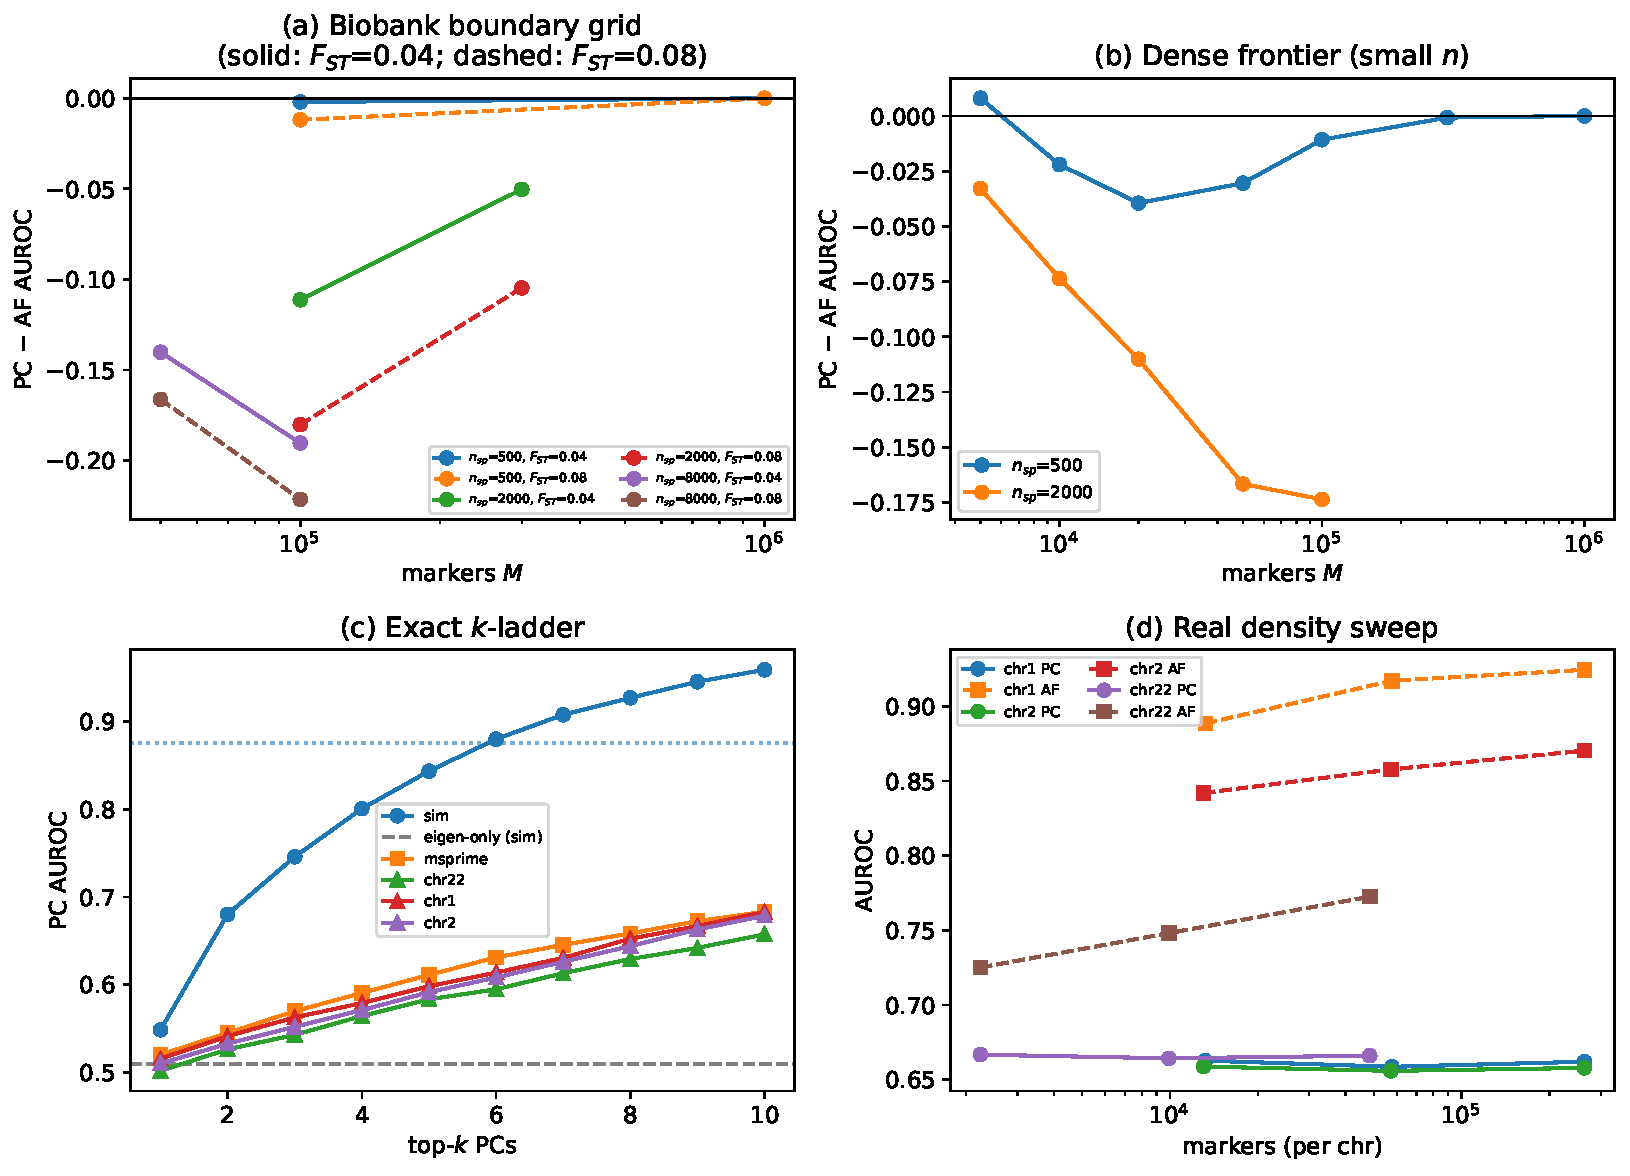
\includegraphics[width=\textwidth]{figures/fig8_scale.pdf}
\caption{Where the ordering lives. (a) Biobank-scale boundary grid. The
PC$-$AF AUROC gap for $n_{\text{sp}}\in\{500,2000,8000\}$; Fst is distinguished
by line style (solid $F_{ST}{=}0.04$, dashed $F_{ST}{=}0.08$), so each curve is a
single condition. The gap is negative for $n_{\text{sp}}\ge 2000$. (b) Dense
small-$n$ frontier: PC leads only
at tiny $M$. (c) Exact $k$-ladder on sim/real/msprime: monotone with decaying
increments, an eigenvalue-only control at chance. (d) Real marker-density sweep:
the PC channel is flat while AF rises, so the gap widens with density.}
\label{fig:scale}
\end{figure}

\section{Discussion: What Governance Must Cover}
\label{sec:discussion}
The results reframe the governance target. Pipelines secure the final summary
statistic while treating diagnostics as free; we show the PC-loading diagnostic
is the larger \emph{intermediate} leak relative to the unconditioned AF-LRT
baseline in the small-$(n{\times}M)$ regime, which
holds on real genomes too (within a population the PC channel dominates AF;
on real data the AF-first switch tracks total study size as well as composition),
and that per-site
frequency release is the largest marginal-frequency single channel. An
in-sample-fitted haplotype/LD table ranks high in its own construction (but a
raw haplotype set is trivially leaking and out of the governed set), and the
batch-associated missingness curve is a confounding control rather than a
release family. A pre-registered reveal
manifest must therefore treat the PC spectrum as a governed object, not a QC
byproduct---and must govern the \emph{loadings}, since within our tested attack
an eigenvalue-only (random-basis) projection, and fixed data-independent bases
including an eigenvalue-weighted one, are at chance ($0.46$--$0.53$) while the full
study-fitted loadings recover the leak. Cross-run, individually
manifest-permitted releases \emph{compose}: a sequence of coarsened single-object
releases (a $\lambda_{GC}$ value, eigenvalues, AF at increasing precision, then
the loadings) raises the cumulative attack AUROC to $0.941$ versus $0.882$ for
the largest single release (5/5 seeds; Fig.~\ref{fig:gov}(c)), so a manifest
needs an explicit anti-composition clause, which our ledger records (from
producer-asserted metadata) as a refinement relation (Section~\ref{sec:governance}).
Measuring a constructed multi-object bundle instead of a declared sequence, a
joint attacker exceeds the strongest single object by $+0.011$ in 5/5 seeds, with
the excess attributable to orthogonal per-individual channels while the
per-panel-constant objects carry no feature for the tested attacker
(Section~\ref{sec:governance}), so the
anti-composition clause must cover composition across channels, not only a single
refinement relation.

\paragraph{Limitations.} Absolute numbers are model-specific and the mechanism's
magnitude is dimensionality-dependent; the PC-dominance ordering is a
small-$(n{\times}M)$ regime property, observed on real 1000G within a population
(gap $+0.05$ to $+0.14$) and switching to AF-first once study size and composition
both grow (Section~\ref{sec:scale}); it also fails at the larger simulated site
sizes of Fig.~\ref{fig:rep}(d), where AF saturates first
(Fig.~\ref{fig:gov}(a) shows the ordering is approximately decreasing in measured structure under
a size-controlled $F_{ST}$ sweep; the real cohorts add a study-size confound
which the scale-matched rerun exposes). A GPU-ported biobank-scale
boundary grid (Section~\ref{sec:scale}) locates the crossover quantitatively.
The biobank-scale cohort arm (a semi-synthetic cohort built from real 1000G
haplotypes, Section~\ref{sec:scale}) reproduces the AF-first ordering at
$n_{\text{sp}}$ up to $16000$ ($48{,}000$ study genomes) with real LD and AF
controls that match the donor library and a relatedness control matched on the
dosage parsimony-phase proxy (on actual copied phase the cohort is more related
than the donor library); the cohort is semi-synthetic,
so its
absolute magnitudes remain model-specific even though its haplotype structure and
proxy relatedness match the donor library.
The quantitative
claims rest on marginal-frequency attacks (likelihood-ratio, correlation, and
learned squared-deviation---forms of the same channel) plus a haplotype/LD
channel and an IBS window-sharing proxy channel. The PC channel requires the study's PC
loadings to be released (as federated PCA shares them); if loadings are withheld
the channel does not apply. Our governance prototype is a plaintext,
release-object-level implementation (manifest, egress monitor, hash-chained
ledger); the \emph{sole-egress binding} is realized as a process-isolation
runtime with a PEP-578 audit hook, a single sanctioned pipe channel, and the
child's stdout/stderr discarded, tested
against the careless-author bypass under a threat model of ordinary Python with
no native code and no root---it is not an MPC/SPU implementation, and a local
user with process control remains outside the model. GPU
acceleration was used only for the leak-measurement kernels; the GPU harness's
rank-based AUROC does not apply midrank tie handling, but a representative
archived cell has zero exact ties (3000/3000 unique scores;
\texttt{s59\_auroc\_tiecheck.py}) and the CPU path uses midrank everywhere, so
the checked values are unaffected. The
biobank-scale simulated cells use a Gaussian diffusion
approximation of the Balding--Nichols per-population frequency draw (matching BN
to $O(\text{Fst}^2)$) and a GPU-side LD construction that differs in detail from
the CPU simulator (a shared latent flipping whole blocks vs.\ CPU per-marker
flips); the exact Beta draw is used in all small-scale cells, and
the independent msprime and real-1000G arms are used as external checks. The
cohort arm is semi-synthetic (mosaic copying from real 1000G haplotypes); the
per-individual metric's per-sample magnitudes are resolution-limited and are
reported as an in-sample, resolution-limited trade-off summary rather than an
absolute privacy guarantee (ordering-only on the real high-AUROC channels).

\bibliographystyle{plainnat}
\begin{thebibliography}{99}
\bibitem[Aherrahrou et al.(2024)]{aherrahrou2024} N. Aherrahrou, H. Tairi, Z. Aherrahrou. Genomic privacy preservation in genome-wide association studies: taxonomy, limitations, challenges, and vision. \emph{Briefings in Bioinformatics}, 2024.
\bibitem[Bu et al.(2021)]{bu2021} D. Bu et al. Haplotype-based membership inference from summary genomic data. \emph{Bioinformatics}, 37(S1):i161, 2021.
\bibitem[Suo et al.(2025)]{fedlmm2025} X. Suo, F. Xue, Y. Zhao. A federated and privacy-preserving framework for large-scale genome-wide association studies with mixed-effects models. bioRxiv, 2025.
\bibitem[Homer et al.(2008)]{homer2008} N. Homer et al. Resolving individuals contributing trace amounts of DNA to highly complex mixtures using high-density SNP genotyping microarrays. \emph{PLoS Genetics}, 4(8):e1000167, 2008.
\bibitem[Laurie et al.(2013)]{rfc6962} B. Laurie, A. Langley, E. Kasper. Certificate Transparency. RFC 6962, IETF, 2013.
\bibitem[Moreau \& Missier(2013)]{prov-o} L. Moreau, P. Missier (eds.). PROV-O: The PROV Ontology. W3C Recommendation, 2013.
\bibitem[Ostrak et al.(2021)]{ostrak2021} A. Ostrak, J. Randmets, V. Sokk, S. Laur, L. Kamm. Implementing privacy-preserving genotype analysis with consideration for population stratification. \emph{Cryptography}, 5(3):21, 2021.
\bibitem[Pascoal et al.(2022)]{pascoal2022} T. A. Pascoal, J. Decouchant, M. V\"olp. Secure and distributed assessment of privacy-preserving GWAS releases (GenDPR). \emph{Middleware}, 2022.
\bibitem[Pascoal et al.(2023)]{igwas2023} T. A. Pascoal, J. Decouchant, C. Fang, et al. I-GWAS: Privacy-preserving interdependent genome-wide association studies. \emph{PoPETs}, 2023(2).
\bibitem[Sankararaman et al.(2009)]{sankararaman2009} S. Sankararaman, G. Obozinski, M. I. Jordan, E. Halperin. Genomic privacy and limits of individual detection in a pool. \emph{Nature Genetics}, 41(9):965--967, 2009.
\bibitem[Shringarpure \& Bustamante(2015)]{shringarpure2015} S. S. Shringarpure, C. D. Bustamante. Privacy risks from genomic data-sharing beacons. \emph{AJHG}, 97(5):631--646, 2015.
\bibitem[Swaminathan et al.(2025)]{ppgwas2025} A. Swaminathan et al. PP-GWAS: Privacy-preserving multi-site genome-wide association study. \emph{Nature Communications}, 2025.
\bibitem[Torres-Arias et al.(2019)]{intoto} J. Torres-Arias et al. in-toto: Providing farm-to-table guarantees for bits and bytes. \emph{USENIX Security}, 2019.
\bibitem[Wagner(2016)]{wagner2016} I. Wagner. Evaluating the strength of genomic privacy metrics. \emph{ACM TOPS}, 2016.
\bibitem[Zari et al.(2022)]{zari2022} O. Zari, J. Parra-Arnau, A. \"Unsal, T. Strufe, M. \"Onen. Membership inference attack against principal component analysis. In \emph{Privacy in Statistical Databases (PSD)}, pp.~269--282, 2022.
\bibitem[Froelicher et al.(2025)]{sfgwas2025} D. Froelicher, H. Cho, M. H. Kang, et al. Secure and federated genome-wide association studies for biobank-scale datasets. \emph{Nature Genetics}, 2025.
\bibitem[Kwatra \& Torra(2023)]{kwatra2023} S. Kwatra, V. Torra. Data reconstruction attack against principal component analysis. In \emph{SocialSec}, 2023.
\bibitem[Lan et al.(2025)]{lan2025} A. Lan, Y. Pawitan, X. Shen. Genomic privacy risks in GWAS summary statistics. medRxiv 2025.09.09.25335252, 2025.
\bibitem[Berrang et al.(2026)]{popets2026} P. Berrang, M. Ryan, K. Wooldridge. Revisiting assumptions for membership inference on summary statistics. \emph{PoPETs}, 2026(4):542--560.
\end{thebibliography}

\end{document}
